\chapter{Анализ предметной области}

    Приложения, работающие с большими объемами данных проникли во все сферы нашей жизни. Банковские системы, бронирование отелей, интернет магазинов --- все они сталкиваются с задачами надежного хранения и обработки больших объемов данных.
    
    \section{Подходы к организации многосерверных систем}
    
        Существует 3 основных подхода к организации систем, состоящих из нескольких вычислительных машин\cite{burger2019distributed}:
        
        \begin{enumerate}
            \item Централизованный
            \item Децентрализованный
            \item Распределенный
        \end{enumerate}
        
        Наиболее простым в организации работы подходом является централизованный. При нем выделяется главный сервер, на который ложится ответственность за управление всем кластером. Зависимые сервера обмениваются сообщениями только с главным сервером и не общаются между собой. Такой подход порождает множество проблем: такими системы являются слабо масштабируемыми и обладают слабой отказоустойчивостью, ведь для приведения системы в неработоспособное состояние достаточно падения только одного главного узла.
        
        Децентрализованный подход пытается решить проблемы централизованного подхода. При нем существуют несколько главных сервером, а так же зависимые от них. Каждых из зависимых серверов общается со своим главным сервером. Такая система является устойчивой к отказу в случае падения одного из главным серверов.
        
        В распределенных системах все узлы системы являются равными, среди нет главных серверов. Каждый из узлов способен обрабатывать запросы. Такая система наиболее устойчива к падению и обладает наилучшей масштабируемостью.
        
        Организация связей в данных подходах изображены на рисунке \ref{fig:cen_dec_dis}.
        
        \begin{figure}
            \centering
            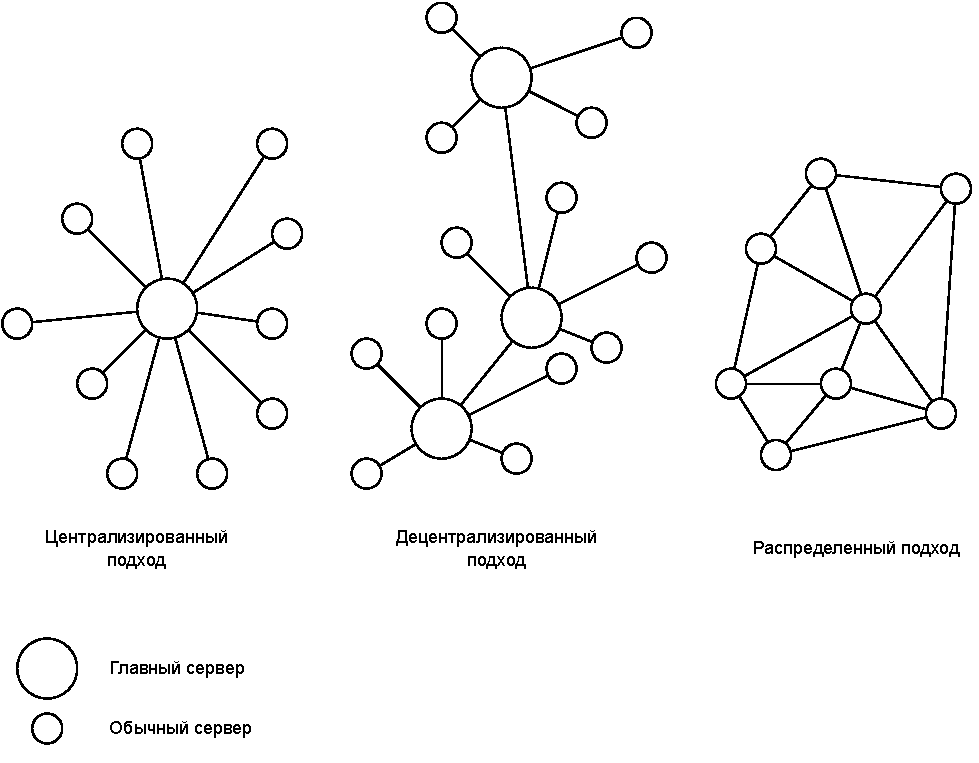
\includegraphics[width=\textwidth*8/10,height=25cm,keepaspectratio]{inc/img/cen-dec-dis.pdf}
            \caption{Организация связей между серверами} \label{fig:cen_dec_dis}
        \end{figure}
        
    \section{Задача достижение консенсуса}

        Фундаментальной проблемой в распределенных системах является достижение общей надежности системы. Для ее достижения необходима координация процессов для достижения общего соглашения по поводу принятия или непринятия некоторого значения всей системой --- задача консенсуса\cite{carlsson1992consensus}. Примерами такой работы может являться соглашение по поводу некоторого единственного значения или задача репликации журнала\cite{panda2018efficient}.
        
        \subsection{Типы отказоустойчивости}
        
            В распределенных системах в работе участвует множество вычислительных машин, каждая из которых может выйти из строя. Рассматривают 2 типа алгоритмов достижения консенсуса по принципу отказоустойчивости:
            
            \begin{itemize}
                \item устойчивость к падению
                \item византийская отказоустойчивость
            \end{itemize}
            
            В первом случае рассматриваются сбои связанные с отказом оборудования, ошибки в программном обеспечении, сбои в сети. Алгоритмы устойчивые к падению не обрабатывают умышленные вредоносные действия в системе. Под византийской же устойчивостью подразумевается обработка в том числе и вредоносных действий узлов: посылка некорректных сообщений, посылка ложной информации, попытка вывести систему из согласованного состояния.
        
        \subsection{Эксклюзивные и инклюзивные алгоритмы}

            Алгоритмы достижения консенсуса классифицируются по модели обеспечения доступа к сети на следующие типы\cite{butun2020review}:
            
            \begin{itemize}
                \item Эксклюзивные
                \item Инклюзивные
            \end{itemize}
            
            В эксклюзивных алгоритмах достижения консенсуса принимать участие в работе алгоритма могут только заранее установленные узлы в ограниченном количестве. В инклюзивных алгоритмах такое ограничение снимается, принимать участие в них может любой желающий узел.
    
    \section{Блокчейн}
    
        Важным толчком в развитии и разработке алгоритмов консенсуса послужило появление криптовалют, построенных поверх технологии блокчейна.
        
        Блокчейн --- выстроенная по определенным правилам непрерывная последовательная цепочка блоков (связный список), содержащих информацию. Связь между блоками обеспечивается не только нумерацией, но и тем, что каждый блок содержит свою собственную хеш-сумму и хеш-сумму предыдущего блока. Изменение любой информации в блоке изменит его хеш-сумму.
        
        Пример цепочки блокчейна приведен на рисунке \ref{fig:blockchain}
        
        \begin{figure}
            \centering
            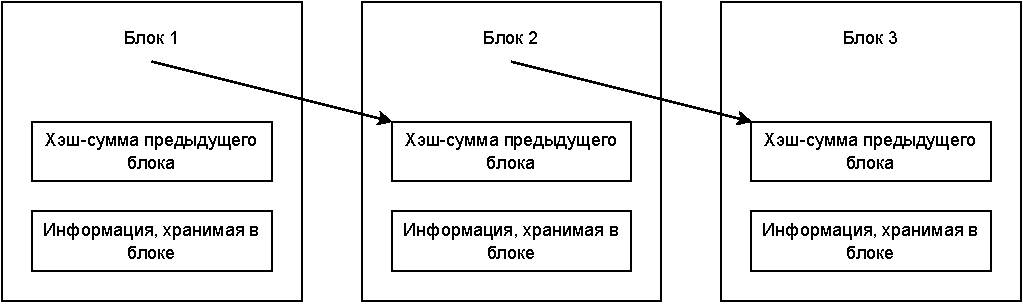
\includegraphics[width=\textwidth*8/10,height=25cm,keepaspectratio]{inc/img/blockchain.pdf}
            \caption{Пример цепочки блокчейна} \label{fig:blockchain}
        \end{figure}
        
    \section{Вывод}

        В данном разделе была обоснована актуальность поставленной задачи, определены основные термины, связанные с алгоритмами достижения консенсуса.